% =====================================================================
% chapters/05_Results.tex — rendu LaTeX de ../traductions/05_results.en_brut.txt (23 septembre 2026)
% Section 5 de la VERSION FRANÇAISE de l'article court. \input depuis main.tex, après 04_Bench.tex.
% Ce fichier DÉFINIT \label{sec:results} et \label{sec:individual}.
% Figures : trois (fig:scale, fig:distance, fig:audit-modes).
% Tableaux : deux (tab:gains, tab:unit).
% Rendu mot pour mot de la traduction fournie par l'auteur.
% =====================================================================

\section{Résultats en régime nominal}
\label{sec:results}

Le régime nominal est une journée ordinaire simulée, celle que décrit l'enquête sur les déplacements des ménages, sans perturbation. Quatre conclusions ressortent de cette journée.

\begin{enumerate}
  \item Les quinze décideurs se répartissent en cinq groupes. Aucun agent génératif n'atteint les quatre références tabulaires.
  \item L'ajustement des critères généraux permet d'aligner certaines dimensions de la distribution, tout en laissant les autres là où il les a trouvées.
  \item Un classificateur typé qui n'écrit aucun texte atteint la même bande, pour un cinquantième du coût.
  \item Deux décideurs que l'agrégat ne permet pas de distinguer sont en désaccord sur un trajet sur trois.
\end{enumerate}

\subsection{Quinze décideurs sur une échelle d'erreur unique}
\label{sec:scale}

Les quinze décideurs se répartissent sur l'axe composite en cinq groupes qui ne se chevauchent pas (Figure~\ref{fig:scale}). Le composite mesurant l'erreur, une valeur plus faible indique une meilleure concordance avec la distribution de l'enquête. Les trois planchers portent l'erreur la plus élevée, de 27,0 pour l'heuristique de durée minimale à 50,2 pour un tirage uniforme sur l'ensemble des choix. Les quatre décideurs sous l'invite minimale se situent entre 7,0 et 14,8. Sous l'invite experte, les trois modèles de langage se situent entre 4,9 et 9,0. Les quatre références tabulaires se tiennent dans un demi-point, de 3,60 à 4,09.

\begin{figure*}[tp]
  \centering
  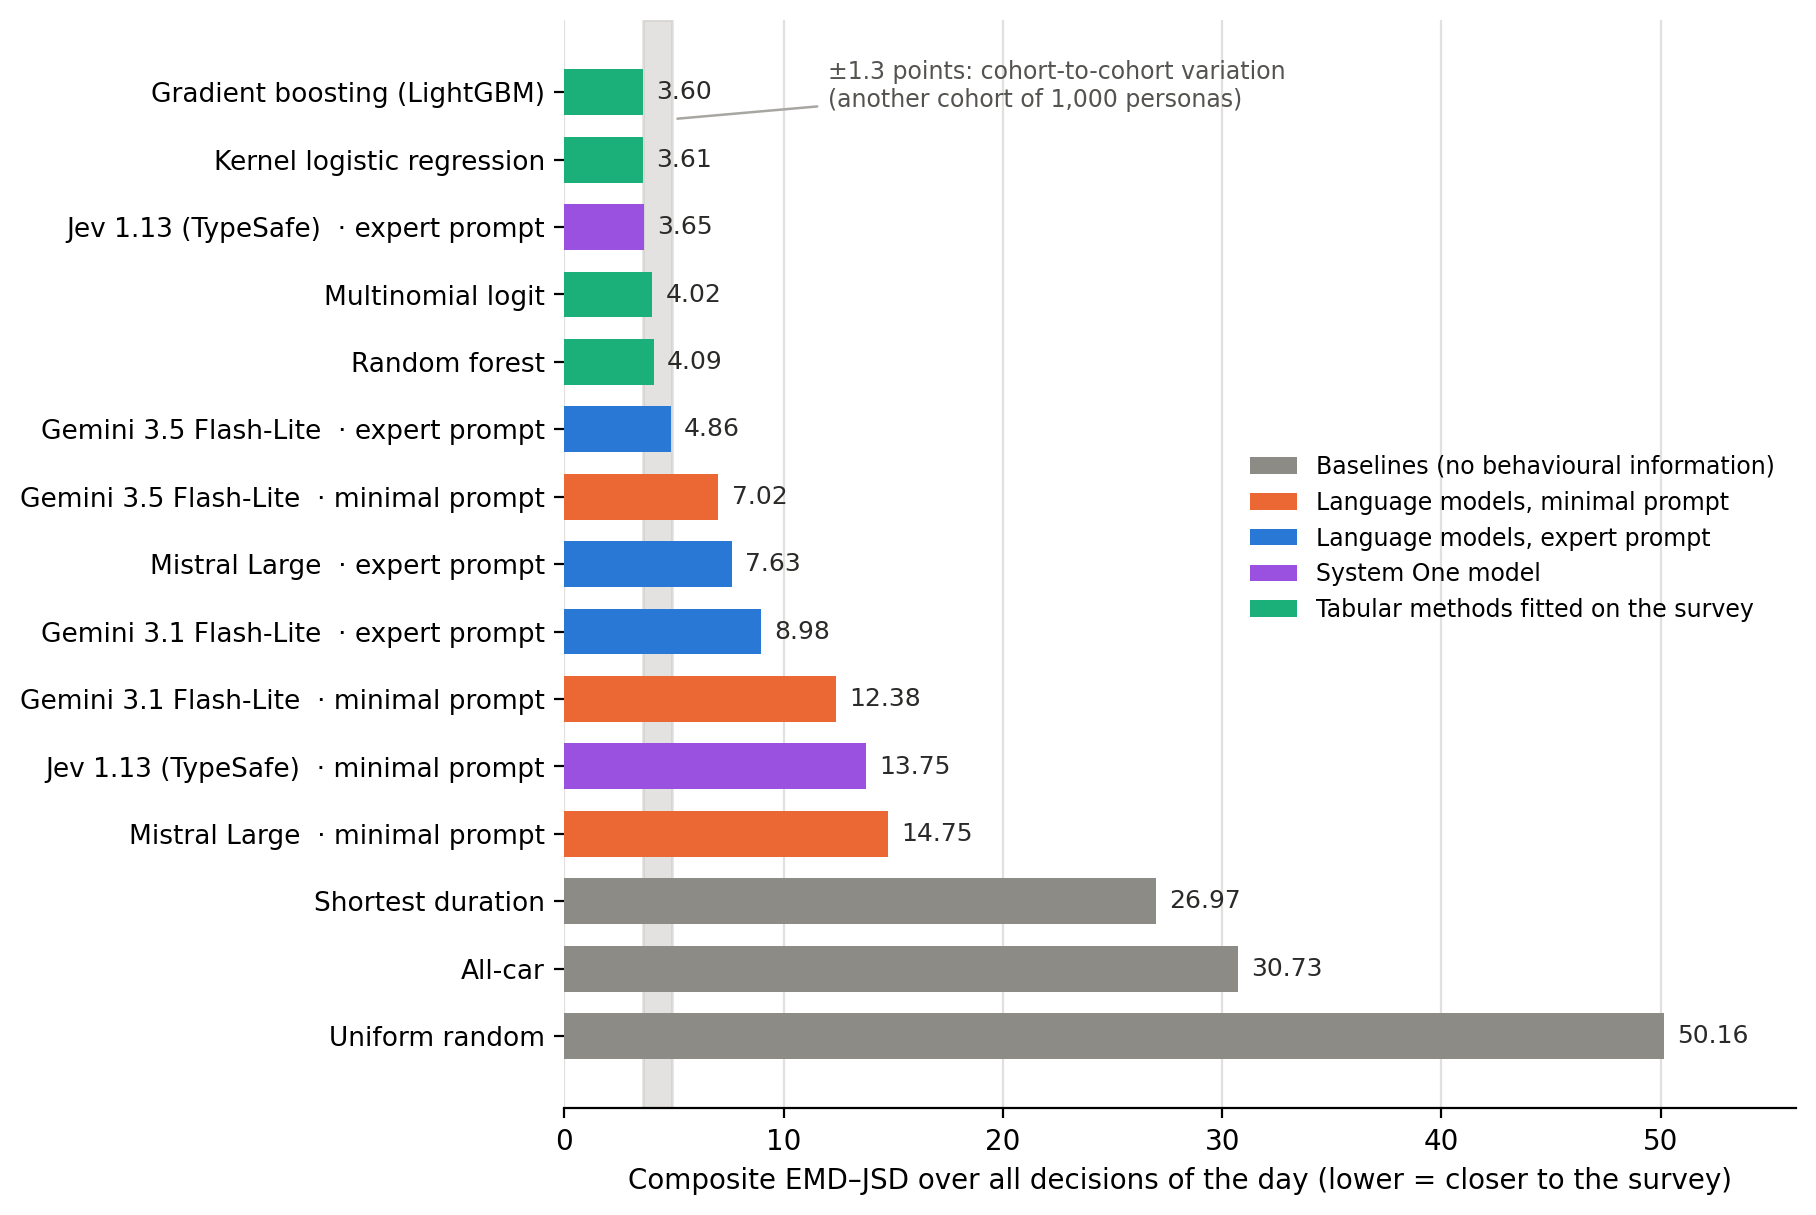
\includegraphics[width=\textwidth]{images/ch6_echelle.png}
  \caption{Cinq groupes se séparent sur l'axe composite, et l'invite minimale présente déjà moins d'erreur que le plancher physique.}
  \Description{Graphique à barres horizontales. L'axe des x représente l'erreur composite EMD-JSD sur chaque décision de la journée, de zéro à gauche à un peu plus de cinquante à droite ; plus la valeur est faible, plus elle est proche de l'enquête. Quinze décideurs sont empilés en lignes et colorés par groupe, chaque barre portant sa valeur. Du meilleur au moins bon : gradient boosting 3,60, régression logistique à noyau 3,61, classificateur typé sous son invite experte 3,65, logit multinomial 4,02 et forêt aléatoire 4,09 ; puis Gemini 3.5 Flash-Lite sous invite experte à 4,86, Gemini 3.5 Flash-Lite sous invite minimale à 7,02, Mistral Large sous invite experte à 7,63, Gemini 3.1 Flash-Lite sous invite experte à 8,98, Gemini 3.1 Flash-Lite sous invite minimale à 12,38, classificateur typé sous invite minimale à 13,75 et Mistral Large sous invite minimale à 14,75 ; à l'extrême droite les trois planchers, plus courte durée à 26,97, tout-voiture à 30,73 et tirage aléatoire uniforme à 50,16. Une bande grise verticale d'environ 1,3 point marque la variation inter-cohortes.}
  \label{fig:scale}
\end{figure*}

L'invite minimale présente déjà moins d'erreurs que le meilleur des trois planchers. La moins bonne des quatre conditions sous invite minimale se situe à 14,8, contre 27,0 pour l'heuristique de durée minimale, qui sélectionne l'option la plus rapide proposée. Un modèle qui reçoit les faits d'un trajet, et aucun critère général, porte donc des informations comportementales. Ces informations ne sont pas celles que l'heuristique physique encode.

Sur deux versions d'une famille de modèles, le modèle de base pèse autant que l'instruction qu'il véhicule. Appliqué sans modification à un second modèle du même fournisseur, le texte expert laisse un écart composite de 4,15 points entre les deux, avec un intervalle de $+$2,99 à $+$5,43.

La réexécution d'une condition avec trois initialisations différentes modifie son score composite de façon moins marquée que la cohorte elle-même. La condition \texttt{gemini-3.5} optimisée obtient des scores de 4,86, 4,65 et 4,30 sur la même cohorte et le même ensemble d'évaluation. L'écart est de 0,56 point, pour une résolution de cohorte de $\pm$1,3 point. Deux autres conditions réexécutées de la même manière présentent des écarts de 0,05 et 0,24 point. Le signe de leur différence est le même pour les trois initialisations.

\subsection{Ce que le réglage influence et ce qu'il n'influence pas}
\label{sec:tuning}

Le réglage des critères généraux améliore chaque modèle de langage, davantage qu'une cohorte ne progresserait seule (Tableau~\ref{tab:gains}). Le gain apparié sur l'axe composite est de 2,27 points pour \texttt{gemini-3.5}, intervalle de $+$1,40 à $+$3,22, puis de 3,37 points pour \texttt{gemini-3.1} et de 7,25 pour \texttt{mistral-large}. Les neuf intervalles excluent zéro. Les gains varient de une fois et demie à cinq fois et demie la résolution de la cohorte.

\begin{table*}[tp]
  \caption{Gains appariés de l'invite experte par rapport à l'invite minimale, trois lectures, avec leur intervalle de confiance à 95\,\% entre crochets. Un gain positif correspond à une erreur plus faible.}
  \label{tab:gains}
  \begin{tabular}{lccc}
    \toprule
    Modèle de langage & Composite & Hors trajets à option unique & L1 sur les parts globales \\
    \midrule
    \texttt{gemini-3.5}    & 2,27 [1,40 ; 3,22] & 3,59 [2,45 ; 4,83]  & 10,2 [8,0 ; 12,5]  \\
    \texttt{gemini-3.1}    & 3,37 [2,45 ; 4,25] & 4,15 [3,09 ; 5,22]  &  8,6 [6,8 ; 10,6]  \\
    \texttt{mistral-large} & 7,25 [5,90 ; 8,67] & 8,63 [7,15 ; 10,28] & 18,0 [13,5 ; 22,4] \\
    \bottomrule
  \end{tabular}
\end{table*}

Ces gains proviennent d'un texte optimisé, et son cheminement n'est pas unique. Chaque mutation déplace plusieurs strates simultanément, dans les deux sens. La procédure ne conserve que les individus dont le mode surreprésenté diminue.

Ce texte crée une pente plutôt qu'un changement de niveau (Figure~\ref{fig:distance}). Sur une distance inférieure à un kilomètre, la part de voiture de \texttt{gemini-3.5} reste stable : 9,7\,\% avant ajustement et 10,1\,\% après. Entre un et cinquante kilomètres, elle augmente de six à sept points dans chaque tranche. L'agent ajusté présente alors une erreur moindre sur la distance que toute référence tabulaire : 14,2 points pondérés contre 16,8 pour la forêt aléatoire. La distance est la seule dimension que l'agent gère.

\begin{figure}[tbp]
  \centering
  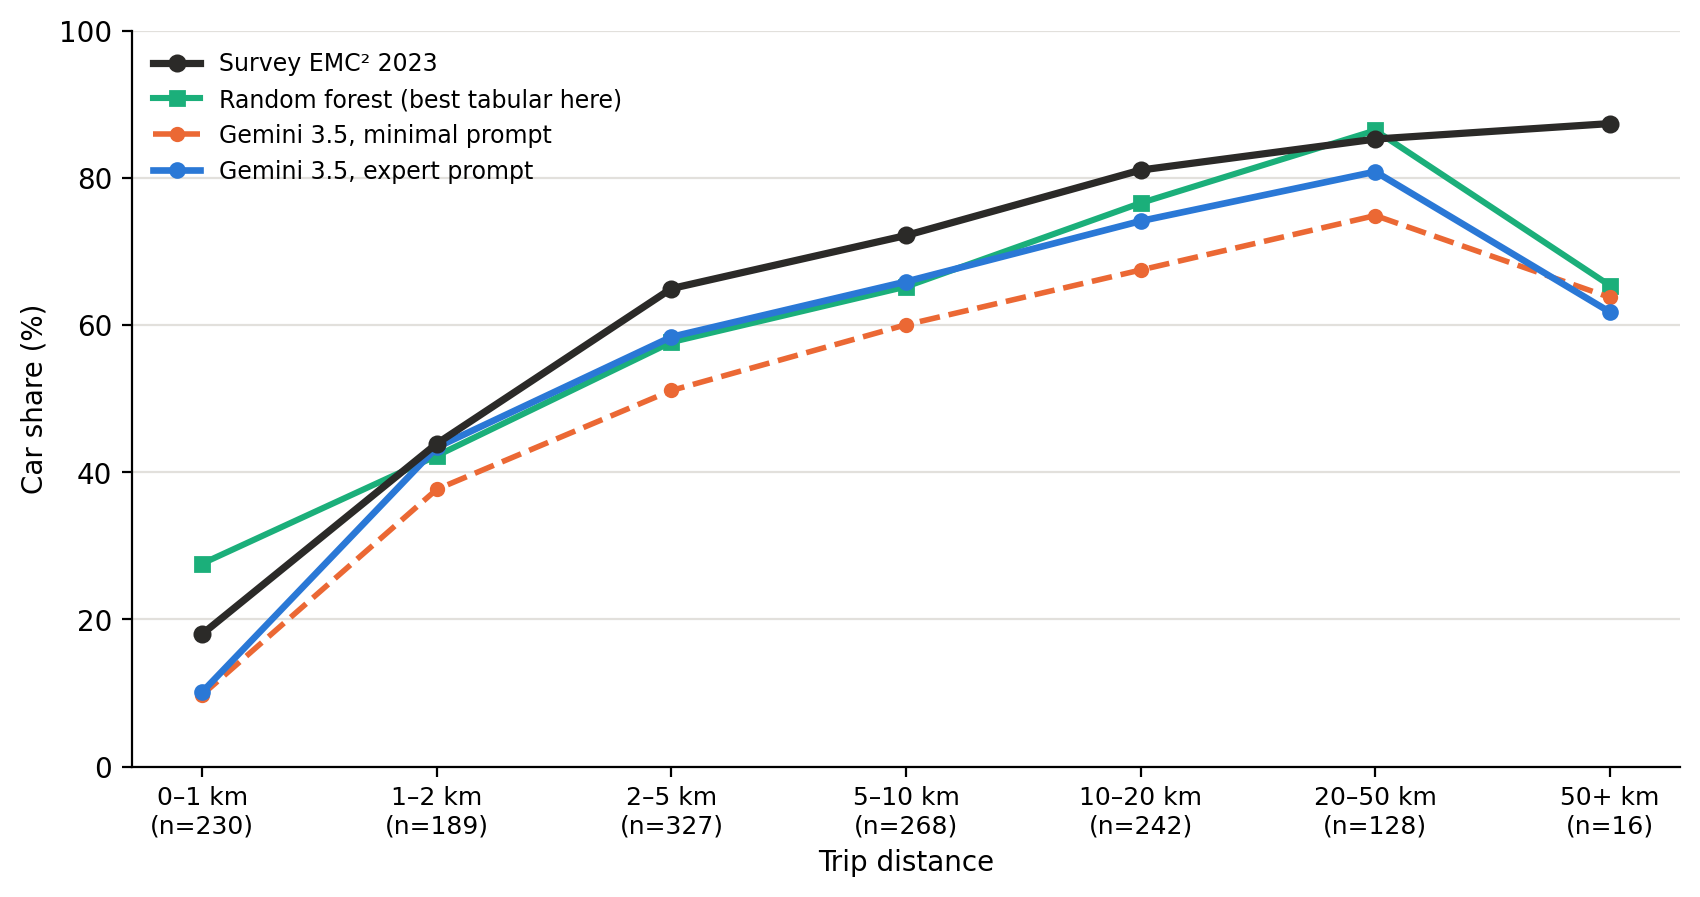
\includegraphics[width=\columnwidth]{images/ch6_distance.png}
  \caption{Le réglage confère à l'agent une pente en fonction de la distance, tandis que les trajets les plus courts restent là où l'invite minimale les a laissés.}
  \Description{Graphique linéaire à quatre séries. L'axe horizontal porte sept tranches de distance de trajet, de zéro à un kilomètre jusqu'à plus de cinquante kilomètres, chacune étiquetée avec son nombre de trajets. L'axe vertical est la part modale de la voiture en pourcentage, de zéro à cent. La courbe de l'enquête monte de 18 pour cent sur la tranche la plus courte à environ 87 pour cent sur la plus longue. L'agent sous invite minimale est le plus bas partout, d'environ 10 pour cent à 75 pour cent. L'agent sous invite experte part des mêmes 10 pour cent mais monte plus vite, rejoignant la forêt aléatoire à partir de deux kilomètres et restant cinq à dix points sous l'enquête.}
  \label{fig:distance}
\end{figure}

Deux erreurs coexistent chez le même décideur, et l'ajustement n'en corrige qu'une. Les trois modèles de langage situent la part de vélo entre 6,8 et 8,1\,\%, alors que l'enquête enregistre 4,1\,\%. Ce texte la modifie de moins d'un point et fait baisser la part des transports en commun de quatre à onze points. Une strate résiste à tous les décideurs : les 15--19 ans (Annexe F).

\subsection{La délibération ne décide pas}
\label{sec:deliberation}

Le classificateur dactylographié atteint la bande des quatre références tabulaires. Son score composite sur la seconde cohorte est \textbf{[c2, score composite hors échantillon du classificateur dactylographié]}, contre 3,60 à 4,09 points pour les quatre références tabulaires. Les différences appariées par rapport à ces quatre références sont \textbf{[c2, quatre différences appariées avec leurs intervalles à 95\,\%]}.

Un décideur qui ne rédige aucun texte obtient un score dans la même bande que ceux qui rédigent une justification. Ce qui aide, c'est donc la lecture du trajet, et non les phrases produites après le choix. La délibération verbalisée n'a rien apporté à la fidélité globale ici. Nous l'affirmons comme un résultat sur ce banc d'essai, et non comme une propriété des modèles de langage.

Pour une charge égale de 23\,026 décisions, le classificateur coûte 1,06 dollar contre 49,28, soit un facteur d'environ cinquante.

\subsection{L'agrégat ne renseigne pas l'individu}
\label{sec:individual}

L'agent optimisé et le modèle à gradient boosté se situent dans la résolution de cohorte l'un de l'autre et divergent encore sur un trajet sur trois. Ils attribuent leur probabilité la plus élevée à un mode différent pour 30,3\,\% des trajets, comptabilisés lorsque les deux ont vu au moins deux options. Cela compare les distributions, et non le mode tiré par chacun. Entre deux méthodes tabulaires, le même chiffre varie de 8,4 à 11,0\,\%. Deux agents diffèrent également quatre fois plus que deux modèles tabulaires sur l'ensemble de la distribution, avec une distance médiane de 40,0 points contre 9,8.

Les jours déclarés de l'enquête, l'agent désigne le mode déclaré légèrement moins souvent que les références tabulaires (Tableau~\ref{tab:unit}). L'audit porte sur 9\,621 trajets de 2\,930 répondants, chacun effectuant le trajet selon le mode déclaré. L'agent optimisé atteint une précision de 67,6\,\% contre 71,5\,\% pour le modèle à gradient boosté, soit un écart de 3,87 points (intervalle : $-$5,47 à $-$2,28). Son écart avec le modèle logit multinomial est significatif, tant en termes de précision que d'entropie croisée.

\begin{table}[tbp]
  \caption{Accord au niveau unitaire sur les jours déclarés, six décideurs. Précision et rappel (\%), entropie croisée sur les 5\,229 décisions prises par chaque décideur (à valeurs distribuées).}
  \label{tab:unit}
  \small
  \setlength{\tabcolsep}{4pt}
  \begin{tabularx}{\columnwidth}{@{}Lrrrr@{}}
    \toprule
    Décideur & \multicolumn{1}{c}{Préc.} & \multicolumn{1}{c}{Entr.} & \multicolumn{1}{c}{Rap.} & \multicolumn{1}{c}{Rap.} \\
             &                           & \multicolumn{1}{c}{crois.} & \multicolumn{1}{c}{vélo} & \multicolumn{1}{c}{marche} \\
    \midrule
    Gradient boosté                      & 71,5 & 0,299 & 20,4 & 63,4 \\
    Logit multinomial                    & 68,6 & 0,358 & 18,3 & 60,0 \\
    Durée minimale                       & 68,1 & ---   & 25,8 & 19,2 \\
    Invite experte, \texttt{gemini-3.5}  & 67,6 & 0,341 & 22,5 & 47,2 \\
    Invite minimale, \texttt{gemini-3.5} & 64,8 & 0,384 & 24,1 & 44,2 \\
    Invite experte, classificateur typé  & 64,7 & 0,464 & 18,1 & 56,3 \\
    \bottomrule
  \end{tabularx}
\end{table}

Le classificateur typé présente une précision individuelle inférieure au seuil minimal pour l'ensemble des véhicules. Il atteint 64,7\,\% là où le plancher atteint 66,7\,\%, soit un écart de 2,04 points (intervalle : $-$3,78 à $-$0,29). Les deux phrases suivantes se basent sur l'invite experte de \texttt{gemini-3.5}, et non sur celle du classificateur lui-même \textbf{[À déterminer]}. Aucune comparaison appariée ne le distingue des quatre références tabulaires sur le composite. Les deux autres lectures agrégées le placent derrière la régression à noyau et la forêt aléatoire. Sa probabilité est plus élevée pour la marche que pour les transports en commun. Le rappel pour la marche est de 56,3\,\%, contre \textbf{[À déterminer, environ 44\,\% sur la Figure~\ref{fig:audit-modes}, valeur exacte dans l'annexe I]} pour les transports en commun. La répartition agrégée masque cette inversion. Une population peut donc reproduire la répartition modale d'un territoire tout en commettant plus d'erreurs sur les trajets individuels qu'une règle qui ne tient pas compte de ces erreurs.

\begin{figure}[tbp]
  \centering
  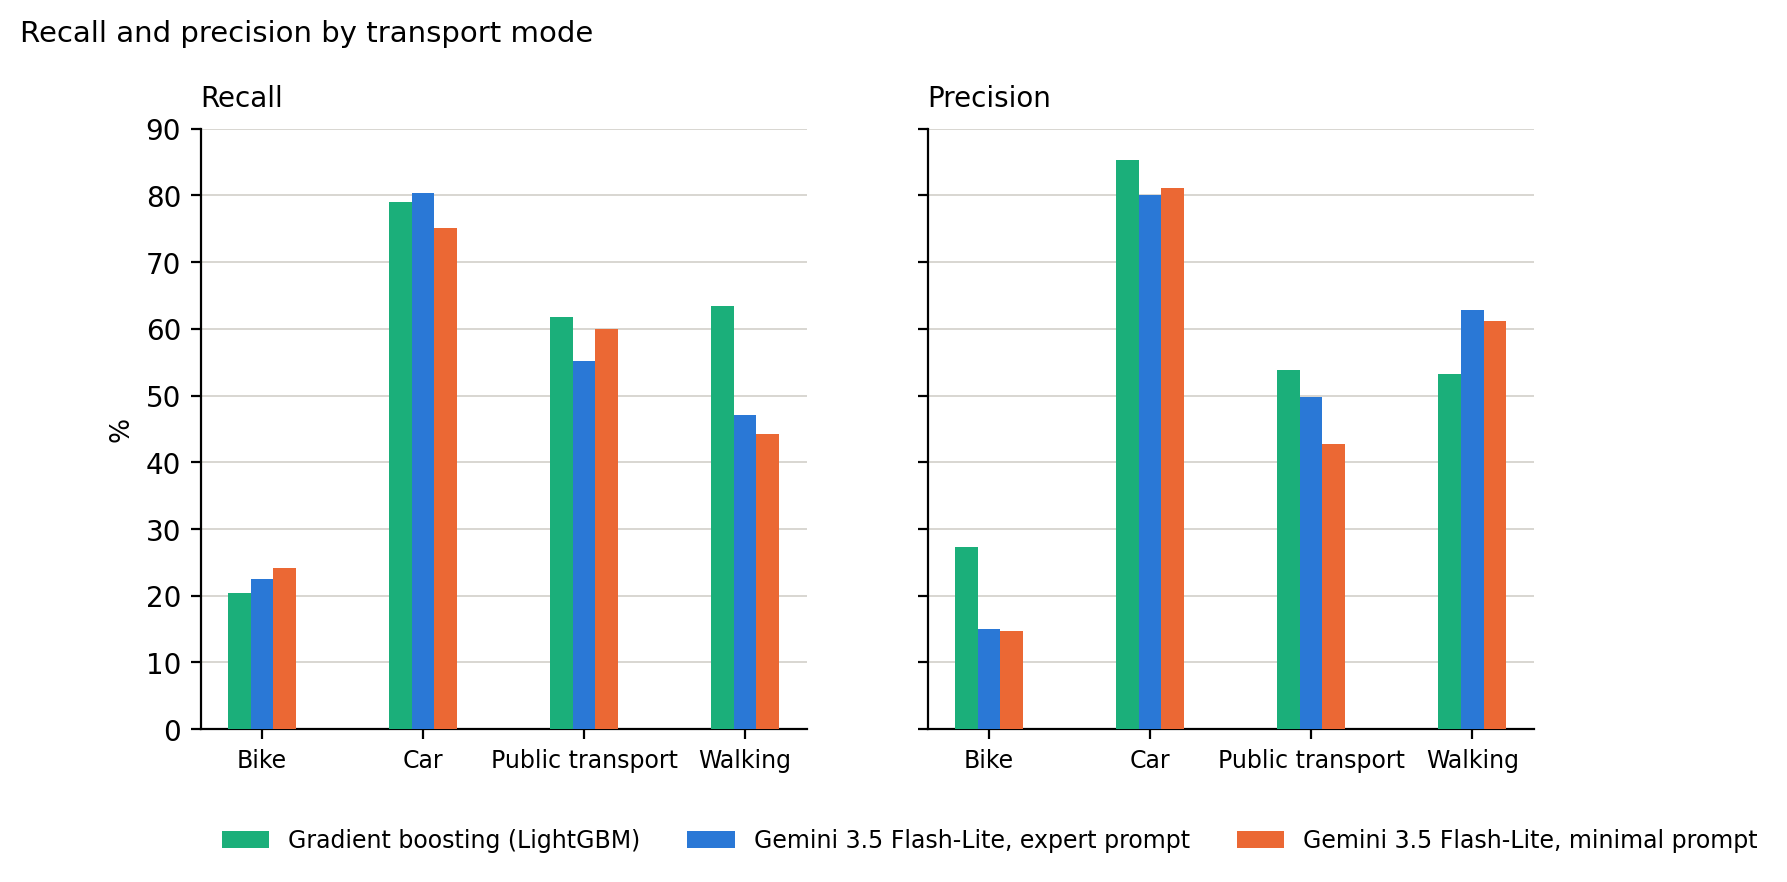
\includegraphics[width=\columnwidth]{images/ch6_audit_modes.png}
  \caption{Rappel et précision par mode : le classificateur typé remplace les transports en commun par la marche et la répartition agrégée ne reflète pas ce changement.}
  \Description{Deux panneaux de barres groupées, rappel à gauche et précision à droite. Dans chaque panneau, l'axe horizontal porte les quatre modes (vélo, voiture, transports en commun et marche), et l'axe vertical un pourcentage de zéro à quatre-vingt-dix. Trois barres par mode : gradient boosting, invite experte sur Gemini 3.5 Flash-Lite, et classificateur typé sous invite experte. Sur le rappel, le classificateur typé est le plus bas sur le vélo et les TC (environ 18 et 44 pour cent), et au-dessus de l'agent génératif sur la marche (56 pour cent contre 47). Sur la précision, la relation s'inverse sur la marche.}
  \label{fig:audit-modes}
\end{figure}

Ces quatre observations sont valables pour la journée ordinaire décrite par l’enquête. Une enquête ne recense aucune autre journée, et la section suivante aborde ce cas de figure pour un événement qu’aucune variable ne permet de modéliser.
